
%-------------------------------------------------------------------------------
% TEMPLATE FOR ITU HWs and Assignments
% (c) Javad Ibrahimli, 2023

% This is a template for a HWs document, created by JAVAD IBRAHIMLI.
% All rights are reserved. 
%------------------------------------------------------------------------------- 


% ------------------ DOCUMENT SETUP ------------------ 
% The document class defines the document type (report) and sets the font size (12pt)
\documentclass[12pt]{report}
\author{Javad Ibrahimli}
\usepackage[backend=biber,style=numeric,sorting=nyt]{biblatex}
\addbibresource{References.bib} % Name of your bibliography file
\usepackage{comment}
\usepackage{pgfplots}
% Inputs the Document Packages
\input{_Packages}

% Controls how many subsections the document can take
%  and how many of those will get put into the contents pages.
\setcounter{secnumdepth}{3}
\setcounter{tocdepth}{3}

% Line Spacing
\setstretch{1.5}


% Places a dot after Chapter/Section/Subsection number in Table of Contents
\renewcommand{\cftchapaftersnum}{.}
\renewcommand{\cftsecaftersnum}{.}
\renewcommand{\cftsubsecaftersnum}{.}

%  Customize Dot spacing in Table of Contents/List of Figures/Tables
\renewcommand{\cftdotsep}{0.3}


% Line Break Properties
\tolerance=1
\emergencystretch=\maxdimen
\hyphenpenalty=10000
\hbadness=10000


% Formatting Table of Contents/Lists titles
\renewcommand{\contentsname}{\bfseries\LARGE{CONTENTS}}
\renewcommand{\listfigurename}{\bfseries\LARGE{LIST OF FIGURES}}

% Signature Line for the declaration
\newbox\namebox
\newdimen\signboxdim

\def\signature#1{%
    \setbox\namebox=\hbox{#1}
    \signboxdim=\dimexpr(\wd\namebox+3cm)
    \parbox[t]{\signboxdim}{%
        \centering
            \hrulefill\\    % for a line
            #1
        \par}%
    }

% Title Formatting customization
\titleformat{\chapter}{\normalfont\bfseries\LARGE}{\thechapter.}{1em}{\MakeUppercase}

\titleformat{\section}{\normalfont\bfseries\large}{\thesection.}{1em}{\MakeUppercase}
\titlespacing*{\section} {0pt} {0pt} {15pt} % left, before, after

\titleformat{\subsection}{\normalfont\bfseries\large}{\thesubsection.}{1em}{}
\titlespacing*{\subsection} {0pt} {10pt} {10pt}

\titleformat{\subsubsection}{\normalfont\bfseries\large}{\thesubsubsection.}{1em}{}
\titlespacing*{\subsubsection} {0pt} {10pt} {10pt}


% HEADER AND FOOTER
\pagestyle{fancy}  % Set Page Style (Header and Footer Style)
\fancyhf{}  % Clears the header and footer (from the default info)

% Header
\renewcommand{\headrulewidth}{0pt}  % Removes the default Horizontal Line in Header
% Optional Headers
%\fancyhead[L]{}
%\fancyhead[R]{2022/2023}

% Footer
\fancyfoot[C]{\thepage} % Page Number

% Change figure numbering per section
\numberwithin{figure}{chapter}

%Acronym entries
\makeglossaries
\newacronym{US}{US}{Ultrasound}



%  -------------------------------------------------
%  --------- The document starts from here --------- 
%  -------------------------------------------------

\begin{document}


% ------------------  TITLE PAGE -------------------

\begin{titlepage}
{\color{purple}
\begin{center}
    
    % UCL IMAGE
    \vspace*{-2.5cm}
    \makebox[\textwidth]{\includegraphics[scale=0.6]{Images/logo_800anni.png}}
    
    \vspace{5cm}
    

    \vspace{1cm}
    {\relscale{1.3}\textbf{Data-Driven Modeling of the Lorenz System Using Physics-Informed Neural Networks\\}}
    \vspace{2.4cm}
    {\relscale{1.35}\textbf{DYNAMICAL SYSTEMS (MOD. B)\\}}
    \vspace{0.3cm}
    
    %\vspace{0.1cm}
    %\vspace{0.1cm}
    Alessandro Crotti \\
    2149762\\
    \vspace{0.9cm}
    {\begin{singlespace}Course given by:\\\end{singlespace}}
    {\begin{singlespace}Antonio Ponno
    \\\end{singlespace}}


\end{center}
{\raggedleft\vfill{\begin{singlespace}
     Department of Civil, Construction and Environmental engineering\\
\end{singlespace}
 Mathematical Engineering\\
 \begin{singlespace}
 % Date of submission: \today\\

 
 \end{singlespace} 
 
}\par
}
}
\end{titlepage}




% ------------------  TABLE OF CONTENTS --------------------
\tableofcontents 


\chapter{Introduction}
Dynamical systems are a cornerstone of mathematical and physical sciences, providing profound insights into how systems evolve over time. Whether studying planetary orbits, stock market fluctuations, or the spread of a virus through a population, dynamical systems offer a robust framework for understanding complex processes. This mathematical concept not only enhances our understanding of the world but also equips us with tools to predict the future behavior of systems under specific conditions. The beauty of dynamical systems lies in their universal applicability, encompassing both deterministic systems—where the future behavior is entirely determined by initial conditions—and stochastic systems, where randomness plays a significant role in the system's evolution.

To study the evolution of such systems, various approaches, known as system identification methods, can be employed. These methods analyze a set of observed or latent states and aim to devise mathematical models to predict the system’s future states. Specifically, for identifying nonlinear dynamics, several deterministic and probabilistic tools are available, including radial basis functions \cite{Chen1990Non-linear}, neural networks \cite{cochocki1993neural}, Gaussian processes \cite{kocijan2005dynamic} \cite{raissi2017hidden} \cite{raissi2017inferring} \cite{raissi2017machine} \cite{raissi2017numerical}, and nonlinear auto-regressive models such as NARMAX \cite{billings2013nonlinear} and recurrent neural networks \cite{goodfellow2016deep}. However, achieving sparse representations of dynamics with these methods often requires the nontrivial task of selecting an appropriate set of basis functions. Thus, expanding the search space for functions is a key area of ongoing research.

In this project, we introduce a novel approach to nonlinear system identification, combining classical multistep time-stepping schemes from numerical analysis with deep neural networks. Inspired by recent advancements in physics-informed neural networks (PINNs), we propose a structured nonlinear regression model capable of uncovering dynamic dependencies from a given set of temporal data snapshots, ultimately returning a closed-form basin of attraction. Unlike recent approaches to system identification, our method does not require direct access to or approximations of temporal gradients, as time derivatives are discretized using traditional time-stepping methods. Additionally, we employ a broader family of function approximators, which eliminates the need to commit to a specific class of basis functions, such as polynomials.

This project is structured as follow. We start with the introduction of the lorenz systems and his chaotic behaviour Chp. \ref{cap: problem}.
In the next capters we will introduced numerical methods used for this problem Chp. \ref{cap: overview}, the problem setup with PINNs Chp. \ref{cap: setup} and code implementation \ref{cap: code}. 




% -------------------  INTRODUCTION  ---------------------
\chapter{Problem}\label{cap: problem}
In this project, I will present an innovative method useful for computing nonlinear systems. In this case, we are interested in the Lorenz system \cite{Lorenz}, as shown in equation \eqref{eq: lorenz}. Particularly, we will study the stability of the system in order to define a set of chaotic solutions of the Lorenz system. These solutions are represented by the Lorenz Attractor.

This model consists of three ordinary differential equations (ODEs).
\begin{equation}\label{eq: lorenz}
\left\{
\begin{aligned}
\frac{dx}{dt} &= \sigma (y - x) \\
\frac{dy}{dt} &= x (\rho - z) - y \\
\frac{dz}{dt} &= x y - \beta z
\end{aligned}
\right.
\end{equation}
Where $\rho$, $\beta$, and $\sigma$ are three positive parameters. $\sigma$ is known as the Prandtl number, and $\rho$ is called the Rayleigh number. $\beta$ is a geometric parameter.

We will employ a method known as the Multistep Physics-Informed Neural Network \cite{PINNs}. It is based on neural network systems that utilize data from different time steps and physical information to approximate the dynamics of the Lorenz Attractor with a limited amount of noisy data.

\section{Lorenz System}
The Lorenz system is a deterministic and chaotic system. It is highly sensitive to initial conditions, making long-term predictions impossible. The system is also symmetric; if $(x(t), y(t), z(t))$ is a solution, then $(-x(t), -y(t), -z(t))$ is also a solution. The dynamics of the system depend on the choice of parameters, especially on the selection of $\rho$, which determines stability. \\In the subsequent study of fixed points, we will explore how this parameter influences stability.

A \textbf{fixed point} is a point in space such that: 
\begin{equation*}
\left\{
\begin{aligned}
0&= \sigma (y - x) &\Longrightarrow &x=y\\ 
0&= x (\rho - z) - y &\Longrightarrow &(\rho-1-z)x=0\\
0&= x y - \beta z &\Longrightarrow &x^2=\beta z
\end{aligned}
\right.
\end{equation*}
A fixed point can be either stable or unstable. We define a stable point as a point in space from which every perturbation decays exponentially. Conversely, for an unstable point, perturbations grow exponentially. This implies that trajectories will either converge to a point $(x, y, z)$ or diverge as $t$ approaches infinity. The parameter $\rho$ plays a crucial role in determining the stability properties of fixed points.

In this case, we have three fixed points. 
\begin{itemize}
    \item $(0,0,0)$ obtained imposing $z$, $y$ or $x$ equal to zero and it is homogeneous for $\rho<1$. 
    \item imposing $z=\rho - 1 \longrightarrow x^2=\beta(\rho-1)$ for $\rho>1$ we obtain two symmetric points $C^{\pm}=(\pm \sqrt{\beta(\rho-1)},\pm \sqrt{\beta(\rho-1)},\rho-1)$ 
\end{itemize}

To study the nature of a fixed point, we are interested in its eigenvalues. If the real parts of the eigenvalues are negative, the fixed point will be stable; otherwise, it will be unstable.

\section{Stability}
The stability of fixed points in a dynamical system can be analyzed by studying the determinant of the Jacobian matrix.

\begin{equation*}
J(x,y,z) = \begin{bmatrix}
\frac{\partial f_1}{\partial x} & \frac{\partial f_1}{\partial y} & \frac{\partial f_1}{\partial z} \\
\frac{\partial f_2}{\partial x} & \frac{\partial f_2}{\partial y} & \frac{\partial f_2}{\partial z} \\
\frac{\partial f_3}{\partial x} & \frac{\partial f_3}{\partial y} & \frac{\partial f_3}{\partial z}
\end{bmatrix} 
= \begin{bmatrix}
-\sigma & \sigma & 0 \\
\rho - z & -1 & -x \\
y & x & -\beta
\end{bmatrix}
\end{equation*}
where $f_1$, $f_2$ and $f_3$ are the three ODEs of the system.


Now, by computing the Jacobian matrix at the fixed point and evaluating its determinant, we can find the eigenvalues. \\
Starting with the \textbf{point $(0,0,0)$}, we obtain:
\begin{equation*}
J(0,0,0) = \begin{bmatrix}
-\sigma & \sigma & 0 \\
\rho & -1 & 0 \\
0 & 0 & -\beta
\end{bmatrix}
\end{equation*}

\begin{equation*}
Det(J(0)-\lambda 1) = Det\begin{bmatrix}
-\sigma-\lambda & \sigma & 0 \\
\rho & -1-\lambda & 0 \\
0 & 0 & -\beta-\lambda
\end{bmatrix} = 0 
\end{equation*}

\begin{equation*}
    \begin{array}{cc}
        (\beta+\lambda) [(\sigma +\lambda)(1+\lambda)-\sigma \rho]=0\\ 
        (\beta+\lambda) [\lambda^2+\lambda(\sigma+1)+\sigma(1-\rho)]=0
    \end{array}
\end{equation*}
So we have find out three eignevalues:
\begin{itemize}
    \item $\lambda_0=-\beta$. Stability requires $\beta >0 $, which is typically the case in the Lorenz system.
    \item $\lambda_{\pm} = \frac{1}{2}[-(\sigma+1)\pm \sqrt{(\sigma-1)^2 +4 \sigma \rho)}]$. We have to study in which conditions the real parts of $\lambda_{\pm}$ are negative. % if: \\$(\sigma-1)^2 +4 \sigma \rho<0$ this inequality implies $\rho <1+\frac{(\sigma-1)^2}{4\sigma}$ 
    In order to do that we define a new matrix
    \begin{equation*}
        A = \begin{bmatrix}
        -\sigma & \sigma  \\
        \rho & -1 \\
        \end{bmatrix} 
    \end{equation*}
    Let's compute the Trace $Tr(A)=-\sigma -1$ and the Determinant of A, $Det(A)=\simga(1-\rho)$. The real part is negative if and only if $$Tr(A)^2<4Det(A)$$
    In Fig. \ref{fig: Poincaré maps}, we can observe the Poincaré map, which provides us with information on the stability criteria: 
\begin{itemize}
    \item For $\rho<1$, we have $Det(A)=\sigma(1-\rho)>0$, implying a stable node in the plane. There are three real negative eigenvalues, and zero acts as a local attractor.
    \item For $\rho>1$, $Det(A)=\sigma(1-\rho)<0$, indicating a saddle in the plane. We observe two real negative eigenvalues and one real positive eigenvalue. Zero becomes an unstable point.
\end{itemize}
For $\rho<1$ every trajectory approaches the origin as $t \longrightarrow \infty$. It is called globally stable.

\end{itemize}








%the determinant is equal to zero if $\lambda_0=-\beta$ or $\lambda_{\pm} = \frac{1}{2}[-(\sigma+1)\pm \sqrt{(\sigma-1)^2 +4 \sigma \rho)}].$ %$\lambda^2+(\sigma+1)\lambda+\sigma(1-\rho)=0 \longrightarrow \lambda_{\pm} = -\frac{1}{2}[(\sigma+1)\pm \sqrt{(\sigma+1)^2 -4 \sigma(1-\rho)}]$ \\ \longrightarrow \sigma(1-\rho) < \frac{(\sigma+1)^2}{4}
%Knowing that there exist three real eigenvalue we want to classify the type of stability. 
%We define a new matrix
%\begin{equation*}
%A = \begin{bmatrix}
%-\sigma & \sigma  \\
%\rho & -1 \\
%\end{bmatrix} 
%\end{equation*}
%We compute the trace of $A$ and the determinant of $A$ as $Tr(A)=-\sigma-1, \ Det(A)=\sigma(1-\rho)$. Knowing that $Tr(A)^2-4Det(A)>0$ it implies $(\sigma+1)^2-4\sigma(1-\rho)>0$

%------------------------------------------------------

\begin{figure}
\centering    
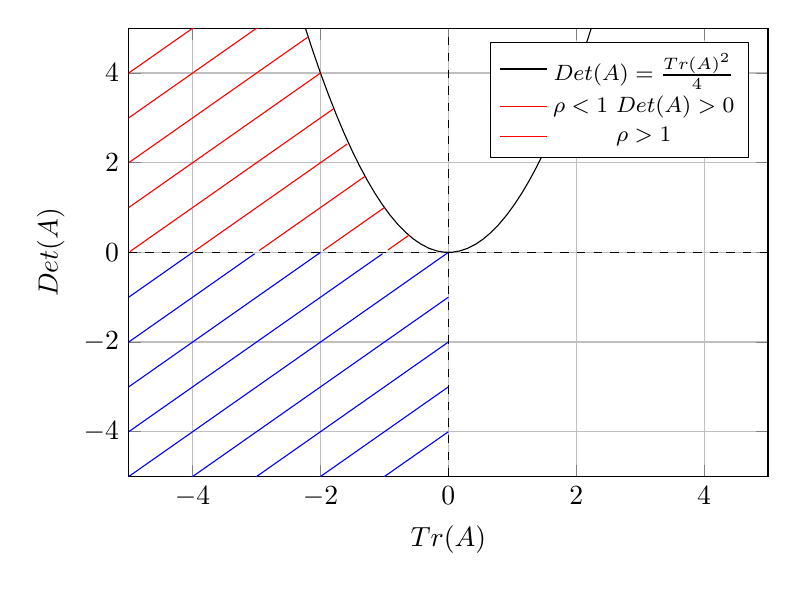
\begin{tikzpicture}
\begin{axis}[
    xlabel={$Tr(A)$},
    ylabel={$Det(A)$},
    grid=major,
    width=0.8\textwidth,
    height=0.6\textwidth,
    xmin=-5, xmax=5,
    ymin=-5, ymax=5,
    legend pos=north east,
    legend style={font=\footnotesize},
    samples=100 % Numero di campioni per disegnare la funzione
]

% Inserisci la tua funzione qui
\addplot[black, domain=-6:6] {x^2};
\addlegendentry{$Det(A)=\frac{Tr(A)^2}{4}$}

\addplot[red,domain=-6:-0.62, restrict y to domain=0:10]{x+1};
\addplot[red,domain=-6:-1, restrict y to domain=0:10]{x+2};
\addplot[red,domain=-6:-1.3, restrict y to domain=0:10]{x+3};
\addplot[red,domain=-6:-1.58, restrict y to domain=0:10]{x+4};
\addplot[red,domain=-6:-1.80, restrict y to domain=0:10]{x+5};
\addplot[red,domain=-6:-2, restrict y to domain=0:10]{x+6};
\addplot[red,domain=-6:-2.2, restrict y to domain=0:10]{x+7};
\addplot[red,domain=-6:-2.58, restrict y to domain=0:10]{x+8};
\addplot[red,domain=-6:-2.58, restrict y to domain=0:10]{x+9};
\addlegendentry{$\rho<1 \ Det(A)>0$}

\addplot[blue,domain=-6:0, restrict y to domain=-10:0]{x-4};
\addplot[blue,domain=-6:0, restrict y to domain=-10:0]{x-3};
\addplot[blue,domain=-6:0, restrict y to domain=-10:0]{x-2};
\addplot[blue,domain=-6:0, restrict y to domain=-10:0]{x-1};
\addplot[blue,domain=-6:0, restrict y to domain=-10:0]{x};
\addplot[blue,domain=-6:0, restrict y to domain=-10:0]{x+1};
\addplot[blue,domain=-6:0, restrict y to domain=-10:0]{x+2};
\addplot[blue,domain=-6:0, restrict y to domain=-10:0]{x+3};
\addplot[blue,domain=-6:0, restrict y to domain=-10:0]{x+4};
\addlegendentry{$\rho>1$}

% Disegna l'asse y=0 e l'asse x=0
\draw[black, dashed] (axis cs:0,\pgfkeysvalueof{/pgfplots/ymin}) -- (axis cs:0,\pgfkeysvalueof{/pgfplots/ymax});
\draw[black, dashed] (axis cs:\pgfkeysvalueof{/pgfplots/xmin},0) -- (axis cs:\pgfkeysvalueof{/pgfplots/xmax},0);

\end{axis}
\end{tikzpicture}
\caption{Stability diagram classifying Poincaré maps}
\label{fig: Poincaré maps}
\end{figure}

%------------------------------------------------------









\vspace{12pt}
%Now suppose $\rho>1$, 
Let's study what happens on the \textbf{points $C^+$ and $C^-$}.
To analyze the stability of these points, we linearize the Lorenz equations around each equilibrium point and compute the Jacobian matrix for the points $C^{\pm}$

\begin{equation*}
J(C^+) = \begin{bmatrix}
-\sigma & \sigma & 0 \\
1 & -1 & - \sqrt{\beta(\rho-1)} \\
\sqrt{\beta(\rho-1)} & \sqrt{\beta(\rho-1)} & -\beta
\end{bmatrix}
\end{equation*}
As we did before, we can determine the eigenvalues computing the following determinant
\begin{equation*}
Det(J(C^+)-\lambda 1) = \begin{bmatrix}
-\sigma -\lambda & \sigma & 0 \\
1 & -1 - \lambda & - \sqrt{\beta(\rho-1)} \\
\sqrt{\beta(\rho-1)} & \sqrt{\beta(\rho-1)} & -\beta - \lambda
\end{bmatrix} = 0 
\end{equation*}

\begin{equation}\label{eq:detC}
    \begin{array}{cc}
         &\lambda^3+(\sigma + \beta +1)\lambda^2+\beta(\rho+\sigma)\lambda + 2\beta\sigma(\rho -1)=f(\lambda)=0
         
    \end{array}
\end{equation}
We can analyze the sign of the eigenvalues graphically. By utilizing software such as Geogebra, we can plot the functions \eqref{eq:detC} and determine the sign by locating their intersections with the y-axis, which varies with $\rho$. In Fig \ref{fig: red and blue lines} we can see a graph like that. The red line describes the case with $\rho=1$ and the blue one with $\rho>1$. In the red case, the intersections with the x-axis tell us that we have 2 distinct negative real eigenvalues and one equal to zero. Otherwise, for $\rho>1$ we find 3 distinct real eigenvalues.




%Let us see what happens if $\rho \longrightarrow 1^+$.
%If $\rho=1 \longrightarrow \lambda[\lambda^2 + (\sigma +\beta+1)\lambda+\beta(1+\sigma)]$. We have three roots
%\begin{itemize}
%    \item $\lambda=0$
%    \item $\lambda_+=-\beta, \lambda_-=-\sigma-1$ %\lambda_{\pm}=\frac{1}{2}[-(\sigma+\beta+1)\pm \sqrt{(\sigma+\beta+1)^2-4\beta(1+\sigma)}]\\=\frac{1}{2}[-(\sigma+\beta+1)\pm \sqrt{(1+\sigma-\beta)^2)}], \
%\end{itemize}
%In Fig. \ref{fig: red and blue lines} we can see a red line for $\rho=1$ and a blue line for $\rho>1$. In the first case, the three intersections with the x-axis tell us that we have 2 distinct real negative eigenvalues and one equal to zero. Otherwise, for $\rho>1$ we find 3 distinct real negative eigenvalues. 
%$\lambda \leq \frac{-2\sigma}{1+\sigma}(\rho-1)$

%------------------------------------------------------
\begin{figure}
\centering    
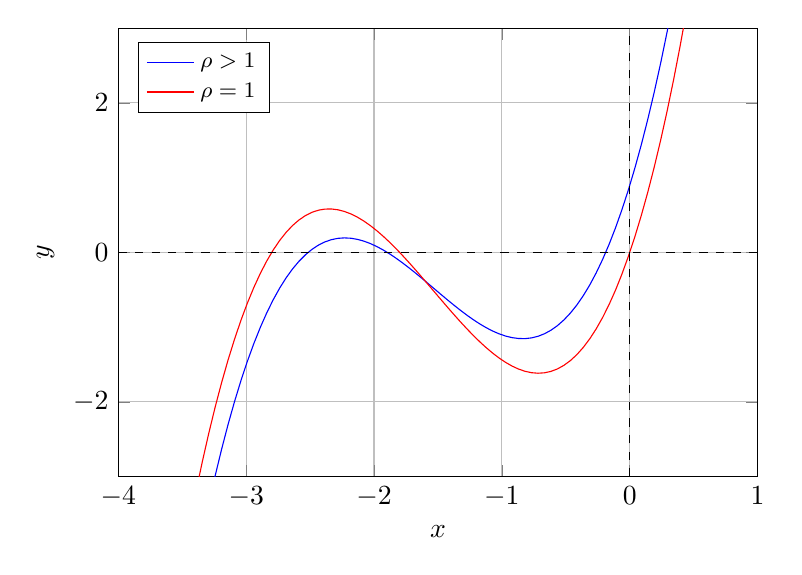
\begin{tikzpicture}
\begin{axis}[
    xlabel=$x$,
    ylabel=$y$,
    grid=major,
    width=0.8\textwidth,
    height=0.6\textwidth,
    xmin=-4, xmax=1,
    ymin=-3, ymax=3,
    legend pos=north west,
    legend style={font=\footnotesize},
    samples=100 % Numero di campioni per disegnare la funzione
]

% Inserisci la tua funzione qui
\addplot[blue, domain=-4:1] {x^3+(0.8+2.8+1)*x^2+2.8*(1.2+0.8)*x+2*0.8*2.8*(1.2-1)}; % Esempio: Grafico della funzione y = x^2
\addplot[red, domain=-4:1] {x^3+(0.8+2.8+1)*x^2+2.8*(1+0.8)*x};
\draw[black, dashed] (axis cs:0,\pgfkeysvalueof{/pgfplots/ymin}) -- (axis cs:0,\pgfkeysvalueof{/pgfplots/ymax});
\draw[black, dashed] (axis cs:\pgfkeysvalueof{/pgfplots/xmin},0) -- (axis cs:\pgfkeysvalueof{/pgfplots/xmax},0);

% Aggiungi la legenda
\legend{$\rho>1$,$\rho=1$}

\end{axis}
\end{tikzpicture}

\caption{$Det (J(C^+)-\lambda 1)=0$ imposing $\rho>1$ and $\rho=1$}
\label{fig: red and blue lines}
\end{figure}

%------------------------------------------------------

\begin{figure}
\centering    
\begin{tikzpicture}
\begin{axis}[
    xlabel=$r$,
    ylabel=$\Bar{x}$,
    grid=major,
    width=0.8\textwidth,
    height=0.6\textwidth,
    xmin=-1, xmax=6,
    ymin=-3, ymax=3,
    legend pos=north west,
    legend style={font=\footnotesize},
    samples=100 % Numero di campioni per disegnare la funzione
]


\draw[dashed,black] (axis cs:0,\pgfkeysvalueof{/pgfplots/ymin}) -- (axis cs:0,\pgfkeysvalueof{/pgfplots/ymax});
\draw[dashed,black] (axis cs:\pgfkeysvalueof{/pgfplots/xmin},0) -- (axis cs:\pgfkeysvalueof{/pgfplots/xmax},0);
\draw[dashed,red] (axis cs:1,0) -- (axis cs:5,0);
% Inserisci la tua funzione qui
\addplot[red, domain=0:1] {0}; % Esempio: Grafico della funzione y = x^2
\addplot[red, domain=-4:4] {sqrt(x-1)};
\addplot[red, domain=-4:4] {-sqrt(x-1)};
\addplot[dashed, red, domain=4:5] {sqrt(x-1)};
\addplot[dashed, red, domain=4:5] {-sqrt(x-1)};
\node[right] at (100,320) {Stable};
\node[right] at (200,420) {Stable};
\node[right] at (200,180) {Stable};
\node[right] at (400,320) {Unstable};
\node[right] at (550,480) {Unstable};
\node[right] at (550,120) {Unstable};
\node[black] at (500,280) {$\rho^*$};
\node[black] at (350,280) {$\rho_0$};
\end{axis}
\end{tikzpicture}

\caption{Stability of the system. When the red lines are dashed the system is unstable. Otherwise it is stable.}
\label{fig: c+}
\end{figure}

%------------------------------------------------------

In Fig, \ref{fig: c+} we can see three stable situation:
\begin{itemize}
    \item $\rho<1$ 
    \item $\rho = 1$ the points $C^{\pm} = (\pm \sqrt{\beta(0)}, \pm \sqrt{\beta(0)}, 0)$ become $(0, 0, 0)$. This value of $\rho$ is significant as it corresponds to a bifurcation point in the Lorenz system.
    \item $1<\rho<\rho^*$ where $\rho^*$ is a critical value of $\rho$ at which one eigenvalue is real and negative while the other two are complex. In this scenario, we can analyze the complex eigenvalues by substituting a generic complex function:
\[
\alpha + i \omega = \text{Tr} \, J(C^+), \quad \text{where} \quad \rho = \rho^*
\]
Here, $\text{Tr} \, J(C^+)$ represents the trace of the Jacobian matrix linearized around the critical point. At $\rho = \rho^*$, we have:
\[
\alpha = -\sigma - 1 - \beta
\]
We define the function $f(\alpha) = f(-\sigma - 1 - \beta)$, which equals zero at $\rho = \rho^*$. Solving this equation for $\rho$, we find:
\[
\rho^* = \sigma \frac{\sigma + \beta + 3}{\sigma - \beta - 1}
\]
where $\sigma - \beta - 1 > 0$ for the expression to be meaningful. This represents a pitchfork bifurcation.
This analysis allows us to understand how the stability of fixed points in the Lorenz system varies with the parameter $\rho$, identifying the critical value $\rho^*$ where a significant bifurcation in the system's behavior occurs.
So, the points $C^{\pm} = (\pm \sqrt{\beta(\rho-1)}, \pm \sqrt{\beta(\rho-1)}, \rho-1)$ are stable only if $\rho^* < \sigma \frac{\sigma + \beta + 3}{\sigma - \beta - 1}$, which is satisfied only for positive values of $\rho$ when $\sigma > \beta + 1$.
\end{itemize}



From the Linear Analysis we have that fixing the parameters $\sigma$ and $\beta$ we can study the eigenvalues varying the parameter $\rho$.
\\How we have just said we have three equilibria $0 \ (\rho<1),C^{\pm} \ (\rho>1)$ and at the point $\rho^*$ the two branches become unstable.
There is another point $\rho_0$
\begin{itemize}
    \item $\rho<\rho_0$ where $C^{\pm}$ are stable nodes
    \item $\rho_0<\rho<\rho^*$ where $C^{\pm}$ are stable spirals
    \item $\rho>\rho^*$ where $C^{\pm}$ are unstable spirals
\end{itemize}
In Fig. \ref{fig: Eigenv} we can see the change in the values of the eigenvalues.

\begin{figure}
    \begin{tikzpicture}
        % Asse x
        \draw[->] (-2,0) -- (2,0) node[right] {$Re$};
        % Asse y
        \draw[->] (0,-2) -- (0,2) node[above] {$Im$};
        % Tre x
        \foreach \x in {-0.5,-1,-1.5}
          \node[black] at (\x,0) {x};
        % Annotazioni
        
        \node[right] at (0.1,1) {3 eigenvalues};
        \node[right] at (-2.3,-0.7) {$1<\rho<\rho_0$};
    \end{tikzpicture}

    \begin{tikzpicture}
        % Asse x
        \draw[->] (-2,0) -- (2,0) node[right] {$Re$};
        % Asse y
        \draw[->] (0,-2) -- (0,2) node[above] {$Im$};
        % Tre x
        \foreach \x in {-1.5}
            \node[black] at (\x,0) {x};
        \filldraw (-0.75,0) circle (2pt);
        % Annotazioni
        
        %\node[right] at (-3,1) {3 eigenvalues};
        \node[right] at (-2.3,-0.7) {$\rho=\rho_0$};
    \end{tikzpicture}
    
    \begin{tikzpicture}
        % Asse x
        \draw[->] (-2,0) -- (2,0) node[right] {$Re$};
        % Asse y
        \draw[->] (0,-2) -- (0,2) node[above] {$Im$};
        % Tre x
        \foreach \x in {-1.5}
            \node[black] at (\x,0) {x};
        \filldraw (-0.75,0.3) circle (2pt);
        \filldraw (-0.75,-0.3) circle (2pt);
        % Annotazioni
        
        \node[right] at (0.1,1) {2 complex conjugate eigenvalues};
        \node[right] at (-2.3,-0.7) {$\rho_0<\rho<\rho^*$};
    \end{tikzpicture}

    \begin{tikzpicture}
        
        % Asse x
        \draw[->] (-2,0) -- (2,0) node[right] {$Re$};
        % Asse y
        \draw[->] (0,-2) -- (0,2) node[above] {$Im$};
        % Tre x
        \foreach \x in {-1.5}
            \node[black] at (\x,0) {x};
        \filldraw (0.75,0.3) circle (2pt);
        \filldraw (0.75,-0.3) circle (2pt);
        % Annotazioni
        
        \node[right] at (0.1,1) {2 complex conjugate eigenvalues};
        \node[right] at (-2.3,-0.7) {$\rho>\rho^*$};
    \end{tikzpicture}
    
    \caption{Caption}
    \label{fig: Eigenv}
\end{figure}

 % Section/Chapter entries can be done in the Main.tex file or in a  
                       % separate tex file for longer and more complex documents

% -------------------  MATERIALS AND METHODS  ---------------------
\chapter{Overview on Physics-Informed Neural Network}\label{cap: overview}
Physics-Informed Neural Networks (PINNs) are a novel and powerful approach to solving differential equations by leveraging neural networks that incorporate the underlying physical laws directly into the learning process. 
\\The typical approach to solve a differential system with a PINNs is to encode the differential equations as part of the loss function during the training process.
\\The main parts that compose a PINNs are:
\begin{itemize}
    \item the neaural networks take as \textbf{input} general information of the system as position $x(t), y(t), z(t)$ and the time step $t$.
    \item The \textbf{Loss function} typically includes: a measure of the difference between the prediction and any available data points like initial condition or Dirichlet/Neumann condition. Here is also inclused a penalization from the Lorenz system equations by evaluating the residuals of the differential equations. This is done by differentiating the neural network outputs with respect to $t$ using automatic differentiation. This one is the \textbf{Physics-informed part}.
    \item The neural network is \textbf{trained} using gradient-based optimization methods, such as Adam Optimization.
\end{itemize}\\
This method presents many advantages respect to the typical numerical methods.
\begin{itemize}
    \item The \textbf{embending of the lorenz equation} into the neural network's loss function, ensure that the learned solution adheres to the underlying physics of the system. This can lead to more accurate and physically consistent solutions, even with limited data.
    \item Once trained, PINNs can potentially \textbf{generalize well} to new conditions or unseen time intervals, provided that the underlying dynamics are well captured during training.
    \item Unlike traditional numerical methods, PINNs don't require discretization of the time or space domain. This make it easier to handle \textbf{complex geometries} or domains.
    \item Another interesting point is that you can use PINNs for solving inverse problems, where the goal is to \textbf{identify unkown parameters} in the differential equations from data. So in the context of the Lorenz system, this could involve estimating parameters like $\sigma, \rho \text{ and } \beta$ directly from the data. 
\end{itemize}\\
Obviously this method has also some disadvantages.
\begin{itemize}
    \item Training a neural network can be \textbf{computationally expensive}. The optimization process involves the evaluation and backpropagation of parameters through the differential equations, which can be resource-intesive.
    \item PINNs can be \textbf{sensitive to the choice of hyperparameteres}, such as the architecture of the neural network such as number of layers and neurons per layer.
    \item The \textbf{quality and quantity of available data} can significantly impact the accuracy of the solution. If the data is sparse or noisy, the network may struggle to learn a precise model.
    \item Unlike traditional numerical methods, which are well-understood and have clear error bounds, PINNs are relatively new, and \textbf{their behavior is not yet fully characterized}.
    \item In chaotic systems like the Lorenz system, where solutions can exhibit high-frequency oscillations or rapid changes, PINNs might \textbf{struggle to capture these dynamics} accurately. This is due to the inherent smoothness of neural networks, which may not naturally represent sharp transitions or high-frequency components. In this project, we will see a particular adaptation of a general PINNs to the Lorenz system. It is called MultistepNNs.
\end{itemize}
 % Section/Chapter entries can be done in the Main.tex file or in a  
                       % separate tex file for longer and more complex documents


% -------------------  MATERIALS AND METHODS  ---------------------
\chapter{Setup and Method} \label{cap: setup}
We are interested in studying a Nonlinear dynamical system of the general form
\begin{equation}\label{eq: general nlds}
    \frac{d}{dt}\boldsymbol{x}(t)=\boldsymbol{f}(\boldsymbol{x}(t)), \ \boldsymbol{x}(t)\in\mathbf{R}^D
\end{equation}
the function $\boldsymbol{f}$ describes the evolution of the system. 
We want to determine the function $\boldsymbol{f}$ and discover the underlying dynamics. In other to do that we start from some measurements of the state $\boldsymbol{x}(t)$ of the system at different time $t_1,t_2,...,t_N$.
Consider the general form of the multistep method with M-steps to equation \ref{eq: general nlds} and obtain
\begin{equation}\label{eq: gen multistep}
\sum_{m=0}^M[\alpha_m\boldsymbol{x}_{n-m}+\Delta t \beta_m\boldsymbol{f}(\boldsymbol{x}_{n-m}]=0, \ n=M,...,N
\end{equation}
where $\boldsymbol{x}_{n-m}$ denotes the state of the system $\boldsymbol{x}(t_{n-m})$.
We will use a neural network (NN) to approximate the function $\boldsymbol{f}$. The parameters of the NN can be learned by minimizing the loss function composed by the mean squared error (MSE) or the sum of the squared error (SSE).
\begin{equation}\label{eq: general loss}
   Loss:=\frac{1}{N-M+1}\sum_{n=M}^N|\boldsymbol{y}_n|^2
\end{equation}
from eq. \eqref{eq: gen multistep} we can define
\begin{equation}\label{eq: gen itearation}
\boldsymbol{y}_n:=\sum_{m=0}^M[\alpha_m\boldsymbol{x}_{n-m}+\Delta t \beta_m\boldsymbol{f}(\boldsymbol{x}_{n-m})], \ n=M,...,N,
\end{equation}
at this point we can redefine the eq. \eqref{eq: general nlds} including the parameterization, time dependence, and forcing
\begin{equation*}
    \frac{d}{dt}\boldsymbol{x}(t)=\boldsymbol{f}(\boldsymbol{x},\boldsymbol{u},t;\lambda), 
 \ \Dot{t}=1, \ \Dot{\lambda}=0
\end{equation*}
where $\boldsymbol{u}(t)$ is the external forcing.

 % Section/Chapter entries can be done in the Main.tex file or in a  
                       % separate tex file for longer and more complex documents
\chapter{Code}\label{cap: code}
Let's break down the Python code step by step.
The original code is available at the following link \hyperlink{https://github.com/maziarraissi/MultistepNNs}{MultistepNNS}

We will use two important libraries: Numpy and TensorFlow. 
\begin{itemize}
    \item Numpy is a fundamental library for scientific computing in Python. While Python itself does not natively support efficient operations on arrays, this library provides powerful tools to manipulate multi-dimensional arrays and perform complex mathematical operations.
    \item TensorFlow is utilized for building and optimizing neural networks. It offers a comprehensive environment for designing machine learning models, allowing for efficient computation and automatic differentiation. This makes it an excellent choice for implementing and training neural networks effectively.
\end{itemize}

Let's focus on the heart of the code, the class:
\begin{verbatim}
class Multistep_NN:
\end{verbatim}
This defines the class \texttt{Multistep\_NN}, which encapsulates the neural network model that is based on a multistep time-stepping scheme for dynamical systems.

\begin{verbatim}
def __init__(self, dt, X, layers, M, scheme):
\end{verbatim}

The class constructor initializes the model with several parameters:
- \texttt{dt}: the time step size.\\
- \texttt{X}: the input data with dimensions $S \times N \times D$, where $S$ is the number of trajectories, $N$ is the number of time snapshots, and $D$ is the number of dimensions in the system.\\
- \texttt{layers}: the structure of the neural network (a list of layer sizes).\\
- \texttt{M}: the number of steps used in the multistep method.\\
- \texttt{scheme}: the multistep method used (Adams-Moulton, Adams-Bashforth, or backward difference formula).

\begin{verbatim}
switch = {'AM': lm.Adams_Moulton, 'AB': lm.Adams_Bashforth, 
         'BDF': lm.backward_difference_formula}
method = switch[scheme](M)
self.alpha = np.float32(-method.alpha[::-1])
self.beta = np.float32(method.beta[::-1])
\end{verbatim}

A dictionary \texttt{switch} is used to select the appropriate numerical method based on the value of \texttt{scheme}. Each scheme is provided by \texttt{nodepy} as a function that takes $M$ steps. The method coefficients \texttt{alpha} and \texttt{beta} are extracted and reversed, to match the time-stepping format. These coefficients are used to combine previous time steps in the multistep method as we have seen in the previous chapter \eqref{eq: gen multistep}.


\begin{verbatim}
self.sess = tf.Session(config=tf.ConfigProto(log_device_placement=True))
self.X_tf = tf.placeholder(tf.float32, shape=[self.S, None, self.D])
self.X_star_tf = tf.placeholder(tf.float32, shape=[None, self.D])
\end{verbatim}

A TensorFlow session \texttt{sess} is created, with logging enabled to show where computations are performed (on CPU or GPU). Two placeholders are defined:
- \texttt{X\_tf} for the full input data of shape $S \times N \times D$.
- \texttt{X\_star\_tf} for a subset of the data used for predictions.

\begin{verbatim}
with tf.variable_scope(scope_name) as scope:
    self.f_pred = self.neural_net(self.X_star_tf)
with tf.variable_scope(scope, reuse=True):
    self.Y_pred = self.net_Y(self.X_tf)
\end{verbatim}

The neural network for prediction (\texttt{f\_pred}) is built using the method \texttt{neural\_net}. The prediction for the time series (\texttt{Y\_pred}) is computed using the multistep method implemented in \texttt{net\_Y}. TensorFlow's variable scope allows reuse of the network parameters for different inputs.

\begin{verbatim}
self.loss = self.D*tf.reduce_sum(tf.square(self.Y_pred))
self.optimizer_Adam = tf.train.AdamOptimizer()
self.train_op_Adam = self.optimizer_Adam.minimize(self.loss)
init = tf.global_variables_initializer()
self.sess.run(init)
\end{verbatim}

The loss function is defined as the sum of squared differences between the predicted values \texttt{Y\_pred} and the true values. This function will be minimized during training. The Adam optimizer is selected for training, and \texttt{train\_op\_Adam} will be used to minimize the loss. All the TensorFlow variables are initialized before the training starts.

\begin{verbatim}
def neural_net(self, H):
    num_layers = len(self.layers)
    for l in range(0,num_layers-2):
        H = tf.layers.dense(inputs=H, units=self.layers[l+1], 
            activation=tf.nn.tanh)
    H = tf.layers.dense(inputs=H, units=self.layers[-1], activation=None)
    return H
\end{verbatim}

This method defines the structure of the neural network. It loops through the specified number of layers (\texttt{num\_layers}). For each layer, it uses \texttt{tf.layers.dense} to apply a fully connected layer. Activation functions (such as \texttt{tanh}) are used to introduce non-linearity. The last layer has no activation function.

\begin{verbatim}
def net_F(self, X):
    X_reshaped = tf.reshape(X, [-1,self.D])
    F_reshaped = self.neural_net(X_reshaped)
    F = tf.reshape(F_reshaped, [self.S,-1,self.D])
    return F
def net_Y(self, X):
    Y = self.alpha[0]*X[:,M:,:] + self.dt*self.beta[0]*self.net_F(X[:,M:,:])
    for m in range(1, M+1):
        Y += self.alpha[m]*X[:,M-m:-m,:] +
             self.dt*self.beta[m]*self.net_F(X[:,M-m:-m,:])
    return Y
\end{verbatim}

\texttt{net\_F} computes the neural network output for the dynamics based on the current data. \texttt{net\_Y} computes the predicted values for each time step using the multistep method with the network-generated dynamics.

\begin{verbatim}
def train(self, N_Iter):
    tf_dict = {self.X_tf: self.X}
    for it in range(N_Iter):
        self.sess.run(self.train_op_Adam, tf_dict)
        if it % 10 == 0:
            loss_value = self.sess.run(self.loss, tf_dict)
            print('It: %d, Loss: %.3e' % (it, loss_value))
\end{verbatim}

This method trains the model for \texttt{N\_Iter} iterations. It updates the model weights using \texttt{train\_op\_Adam} and prints the loss every 10 iterations.

\begin{verbatim}
def predict_f(self, X_star):
    F_star = self.sess.run(self.f_pred, {self.X_star_tf: X_star})
    return F_star
\end{verbatim}

This method uses the trained network to predict the dynamics for a given input \texttt{X\_star}. It returns the predicted output \texttt{F\_star}.

This script defines a neural network model that approximates the dynamics of a system using a multistep time-stepping method. The model is trained using observed time series data, and the resulting network can predict future states of the system.


% -------------------  MATERIALS AND METHODS  ---------------------
\chapter{Results}
This section analyzes the performance of different neural network configurations applied to the Lorenz system. All data in this section is generated using the following settings:
\begin{itemize}
    \item \textbf{BDF Scheme} (Backward Differentiation Formula)
    \item \textbf{M = 3}: Order of the BDF scheme
    \item \textbf{Skip = 1}: Time step interval used between evaluations
    \item \textbf{Number of iterations = 50,000}: Maximum training iterations
    \item \textbf{Initial Position}: The trajectory calculations start from a given initial position in the Lorenz system $x = -8.0, y = 8.0, z = 27$.
    \item \textbf{System parameters}: $\sigma = 10.0$, $\beta = 8.0/3.0$ and $\rho = 28.0$.
\end{itemize}

The experiments involve neural networks with 5 layers and varying neurons per layer (40, 60, 80, and 100). For each configuration, we observe errors along the \( x \), \( y \), and \( z \) axes of the Lorenz attractor, as well as the minimum and last loss values.

\section{Analysis of Neural Network Structure}
\subsection{Error Analysis}

Table \ref{tab:error} shows the errors for each configuration along each axis:

\begin{center}\label{tab:error}
\begin{tabular}{|c|c|c|c|}
\hline
Neurons per Layer & \( \text{Error}_x \) & \( \text{Error}_y \) & \( \text{Error}_z \) \\
\hline
40 & 1.4029 & 1.3886 & 0.4453 \\
60 & 1.2870 & 1.2966 & 0.5114 \\
80 & 1.2897 & 1.3255 & 0.4813 \\
100 & 1.2540 & 1.2523 & 0.4795 \\
\hline
\end{tabular}
\end{center}

\noindent
Errors along the \( x \) and \( y \) axes generally decrease as the number of neurons increases, suggesting that higher neuron counts improve the network’s ability to capture the dynamics along these dimensions. However, the reduction in error becomes less significant beyond 60 neurons, indicating diminishing returns. The error on the \( z \)-axis is lower and stabilizes with configurations of 80 neurons and above, possibly because the \( z \)-dimension is simpler for the model to approximate. In Fig. \ref{fig:trajectory_comparison}, we observe that the model captures the system's behavior effectively. Although the error may seem relatively large, the neural network successfully learns the essential dynamics of the system.

\begin{figure}[h!]
    \centering
    \includegraphics[width=0.8\textwidth]{Images/80x5.png}
    \caption{Comparison of the true and predicted trajectories along the \( x \), \( y \), and \( z \) axes with a $80\text{x}5$ configuration. This illustrates how well this model can capture the behavior of the system.}
    \label{fig:trajectory_comparison}
\end{figure}

\subsection{Loss Analysis}
The minimum and last loss values, representing the lowest and final values of the loss function during training, indicate the network’s convergence behavior and accuracy. 

\begin{center}
\begin{tabular}{|c|c|c|}
\hline
Neurons per Layer & Minimum Loss & Last Loss \\
\hline
40 & 0.0172 & 0.4329 \\
60 & 0.0087 & 0.0151 \\
80 & 0.0063 & 0.0068 \\
100 & 0.0052 & 0.0398 \\
\hline
\end{tabular}
\end{center}

\noindent
The minimum loss consistently decreases with larger networks, showing that higher neuron counts help the network reach lower loss values during training. The last loss value is close to the minimum loss for configurations of 60 and 80 neurons, indicating stable convergence. Interestingly, the 100x5 configuration shows a higher last loss (0.0398), which may suggest overfitting or instability in the training process for networks of this size.

\begin{figure}[h!]
    \centering
    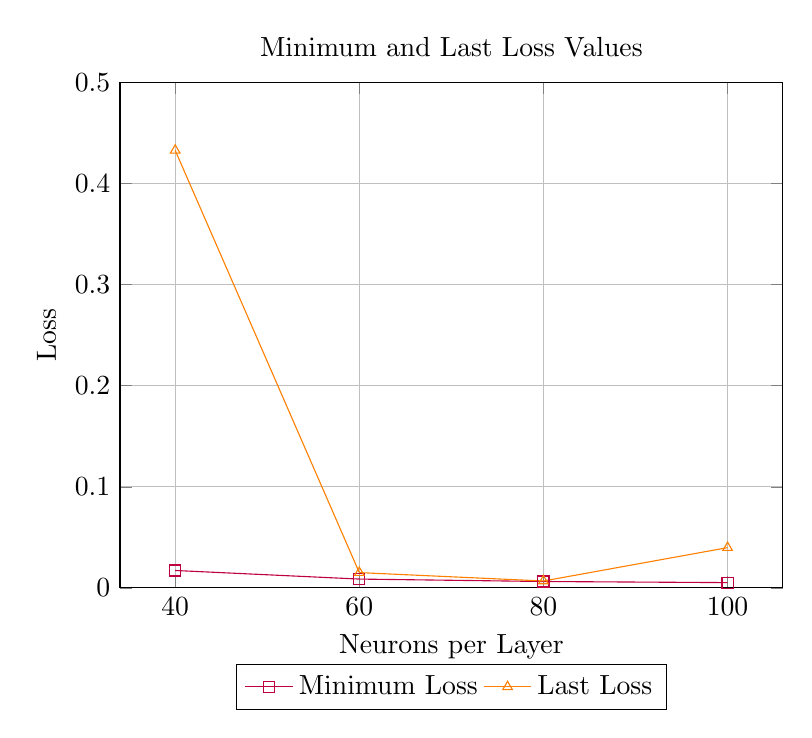
\begin{tikzpicture}
        \begin{axis}[
            width=10cm, height=8cm,
            xlabel={Neurons per Layer},
            ylabel={Loss},
            xtick={40, 60, 80, 100},
            legend style={at={(0.5,-0.15)}, anchor=north, legend columns=-1},
            ymin=0, ymax=0.5,
            grid=both,
            title={Minimum and Last Loss Values}
        ]
        % Minimum Loss
        \addplot[color=purple, mark=square] coordinates {
            (40, 0.0172)
            (60, 0.0087)
            (80, 0.0063)
            (100, 0.0052)
        };
        \addlegendentry{Minimum Loss}

        % Last Loss
        \addplot[color=orange, mark=triangle] coordinates {
            (40, 0.4329)
            (60, 0.0151)
            (80, 0.0068)
            (100, 0.0398)
        };
        \addlegendentry{Last Loss}
        \end{axis}
    \end{tikzpicture}
    \caption{Minimum and last loss values for different network configurations.}
    \label{fig:loss_plot}
\end{figure}

Fig. \ref{fig:loss_plot} illustrates the oscillatory behavior of the loss function during optimization. In this way, After a finite number of iterations, we may reach a local maximum, resulting in a lower optimization level (higher loss), or a minimum, achieving a higher optimization level (lower loss). Setting a minimum error threshold is recommended. However, the solution may still fail to converge, potentially resulting in additional iterations without significant improvement and increased computational expense. 



\section{Analysis of Parameter \( M \)}
This analysis is done using the $80 \times 5$ configuration and varying the value of \( M \) between 1 and 5.


\subsection{Loss Function Analysis Varying \( M \)}

To better illustrate the convergence behavior as \( M \) varies, Figure \ref{fig:loss_M} shows the minimum and last loss values for each \( M \) value. As observed, there is a general trend of decreasing last loss with increasing \( M \), indicating improved model convergence as \( M \) increases.

\begin{figure}[h!]
    \centering
    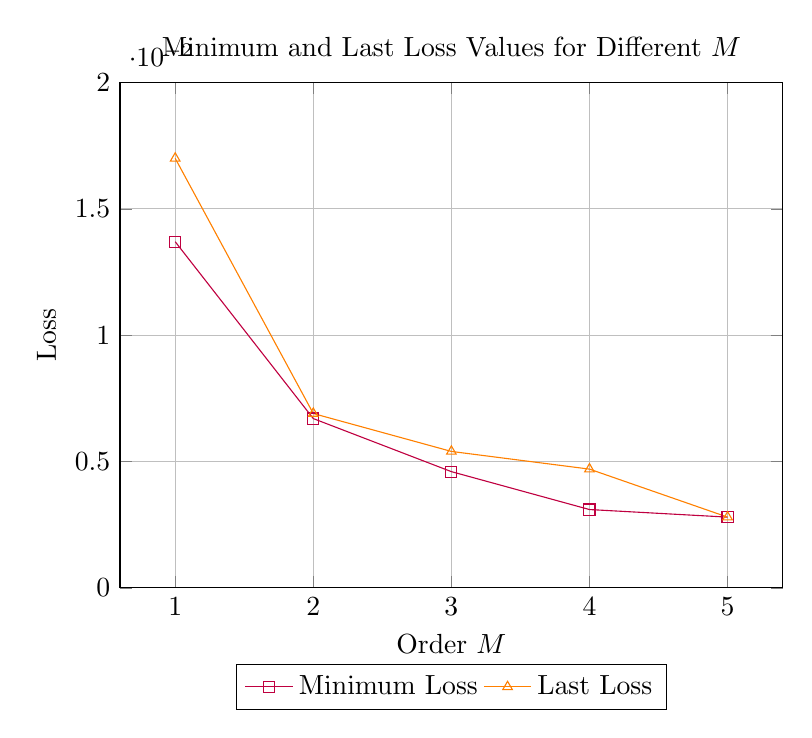
\begin{tikzpicture}
        \begin{axis}[
            width=10cm, height=8cm,
            xlabel={Order \( M \)},
            ylabel={Loss},
            xtick={1, 2, 3, 4, 5},
            legend style={at={(0.5,-0.15)}, anchor=north, legend columns=-1},
            ymin=0, ymax=0.02,
            grid=both,
            title={Minimum and Last Loss Values for Different \( M \)}
        ]
        % Minimum Loss
        \addplot[color=purple, mark=square] coordinates {
            (1, 0.0137)
            (2, 0.0067)
            (3, 0.0046)
            (4, 0.0031)
            (5, 0.0028)
        };
        \addlegendentry{Minimum Loss}

        % Last Loss
        \addplot[color=orange, mark=triangle] coordinates {
            (1, 0.0170)
            (2, 0.0069)
            (3, 0.0054)
            (4, 0.0047)
            (5, 0.0028)
        };
        \addlegendentry{Last Loss}
        \end{axis}
    \end{tikzpicture}
    \caption{Minimum and last loss values as a function of \( M \).}
    \label{fig:loss_M}
\end{figure}

\subsection{Error Analysis Varying \( M \)}

Figure \ref{fig:error_M} presents the errors in the \( x \), \( y \), and \( z \) directions for each value of \( M \). We observe a reduction in errors with increasing \( M \), particularly along the \( z \)-axis, suggesting that higher values of \( M \) contribute to a more accurate approximation of the solution, especially along certain dimensions.

\begin{figure}[h!]
    \centering
    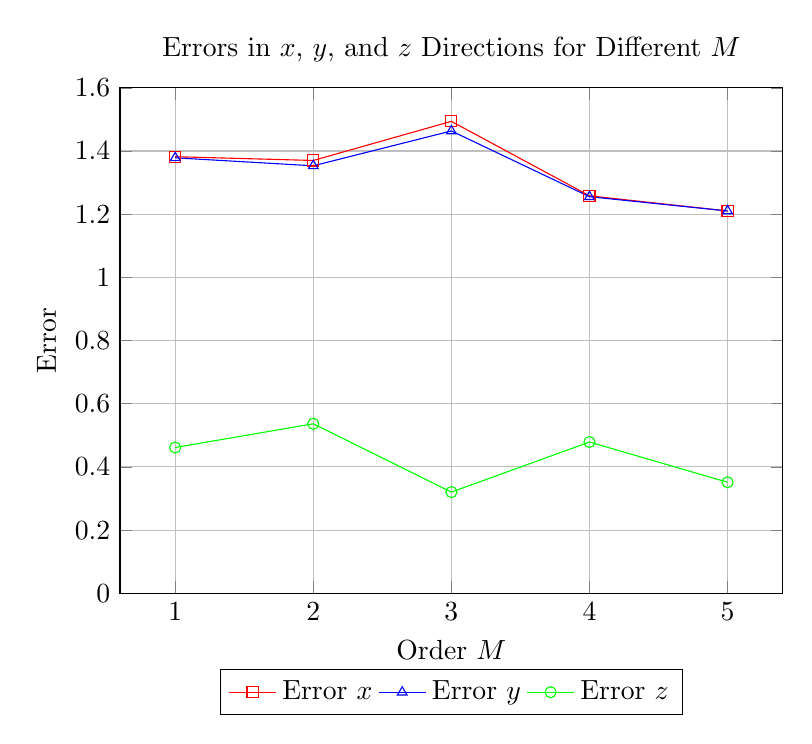
\begin{tikzpicture}
        \begin{axis}[
            width=10cm, height=8cm,
            xlabel={Order \( M \)},
            ylabel={Error},
            xtick={1, 2, 3, 4, 5},
            legend style={at={(0.5,-0.15)}, anchor=north, legend columns=-1},
            ymin=0, ymax=1.6,
            grid=both,
            title={Errors in \( x \), \( y \), and \( z \) Directions for Different \( M \)}
        ]
        % Error_x
        \addplot[color=red, mark=square] coordinates {
            (1, 1.3821)
            (2, 1.3702)
            (3, 1.4940)
            (4, 1.2583)
            (5, 1.2103)
        };
        \addlegendentry{Error \( x \)}

        % Error_y
        \addplot[color=blue, mark=triangle] coordinates {
            (1, 1.3786)
            (2, 1.3533)
            (3, 1.4636)
            (4, 1.2554)
            (5, 1.2103)
        };
        \addlegendentry{Error \( y \)}

        % Error_z
        \addplot[color=green, mark=o] coordinates {
            (1, 0.4615)
            (2, 0.5365)
            (3, 0.3203)
            (4, 0.4788)
            (5, 0.3514)
        };
        \addlegendentry{Error \( z \)}
        \end{axis}
    \end{tikzpicture}
    \caption{Errors along the \( x \), \( y \), and \( z \) directions as a function of \( M \).}
    \label{fig:error_M}
\end{figure}

\subsection{Summary of \( M \) Analysis}

From the above plots, it is evident that increasing \( M \) leads to a decrease in both the last loss and errors, with some variability across the \( x \), \( y \), and \( z \) components. These results suggest that optimizing the parameter \( M \) could play a critical role in improving the model's accuracy and efficiency in future applications.


\section{Comparison with Traditional Numerical Methods}

There exist many numerical methods, each useful in different situations. Each method has its own advantages and disadvantages, and its utility depends on the specific context and problem being addressed.

In general, numerical methods can be challenging to implement. They require complete knowledge of the system's parameters and usually work within simple domains. When studying dynamical systems, a numerical method may lose accuracy over long time periods, accumulating errors at each iteration. In contrast, a well-trained PINN could capture the system's behavior and provide a more accurate long-term solution.

While training a PINN can be costly in terms of time and computational resources, a properly trained PINN can generalize the system's dynamics and predict different solutions under varying parameters. This approach represents an innovative method that combines our understanding of neural networks with traditional numerical methods. Although it may not always achieve the same accuracy and can sometimes be more computationally expensive, its potential is remarkable.

\section{Conclusion}

In summary, increasing the number of neurons per layer generally reduces the error and minimum loss, indicating improved performance. However, the diminishing returns on errors along \( x \) and \( y \) suggest that further increases may not yield significant gains. The 80x5 configuration provides a good balance between accuracy and stability, while the 100x5 configuration shows signs of overfitting or instability, as indicated by the increased last loss. 

Similarly, increasing \( M \) results in lower errors and improved convergence, emphasizing its importance in optimizing the PINN for this system.


 % Section/Chapter entries can be done in the Main.tex file or in a  
                       % separate tex file for longer and more complex documents



\printbibliography[title={References}]



\end{document}
%  -------------------------------------------------
%  --------- The document ends from here ----------- 
%  -------------------------------------------------
